\chapter{Schiemannen}
\vspace{-120px}
\question{1}{Met welke knoop maak je twee touwen van ongelijke dikte aan elkaar vast?}
\answerTextFour{Schootsteek}{Paalsteek}{Constrictor}{Platte knoop}

\question{2}{Welke knoop zie je in de afbeelding hiernaast?}
	\vspace{-20px}
\begin{figure}[H]	

	\begin{minipage}[]{0.70\textwidth}
		\begin{enumerate}[topsep=0pt, label=\Alph*.]
			\item Een achtknoop
			\item Een platte knoop
			\item Een halve steek
			\item Een schootsteek
		\end{enumerate}
	\end{minipage}
	\begin{minipage}[]{0.29\textwidth}
		\begin{figure}[H]
			
\includegraphics[width=0.80\textwidth,right]{Hoofdstukken/Schiemannen/pdf/platteknoop.pdf}
		\end{figure}
	\end{minipage}
	\vspace{-20px}
\end{figure}


\question{3}{Welke knoop leg je op een mastworp als iets voor lange tijd vast moet blijven?}
\answerTextFour{Halve steek}{Achtknoop}{Schootsteek}{Slipsteek}

\question{4}{Welke knoop laat een halve steek zien?}
\begin{figure}[H]
	\centering
	\begin{minipage}[b]{0.23\textwidth}
		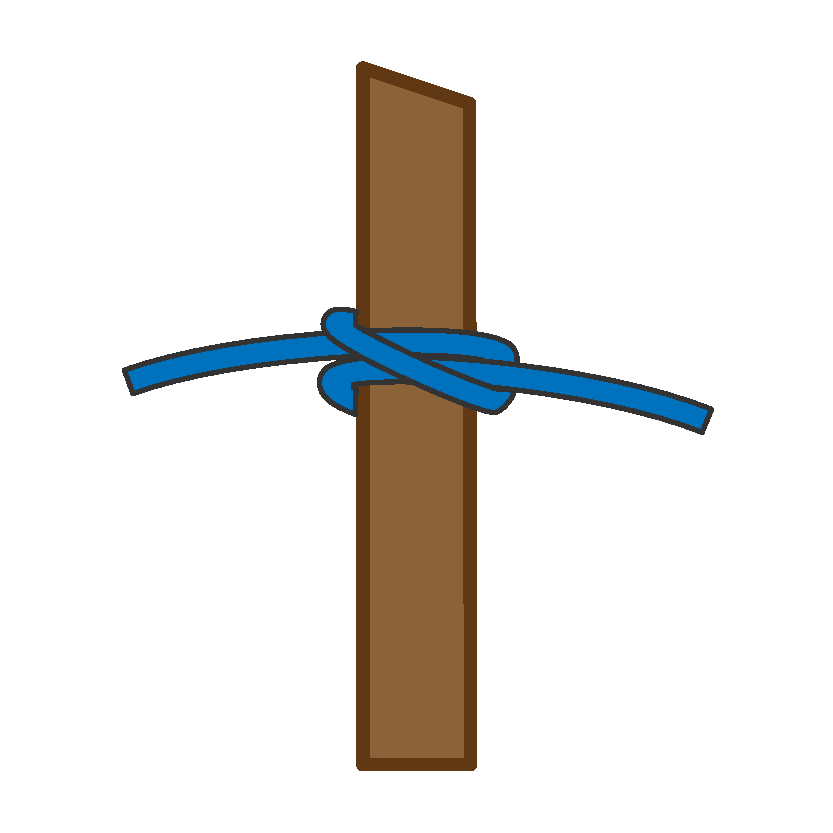
\includegraphics[width=\textwidth]{Hoofdstukken/Schiemannen/pdf/mastworp.pdf}
		\centering
		A
	\end{minipage}
	\hfill
	\begin{minipage}[b]{0.23\textwidth}
		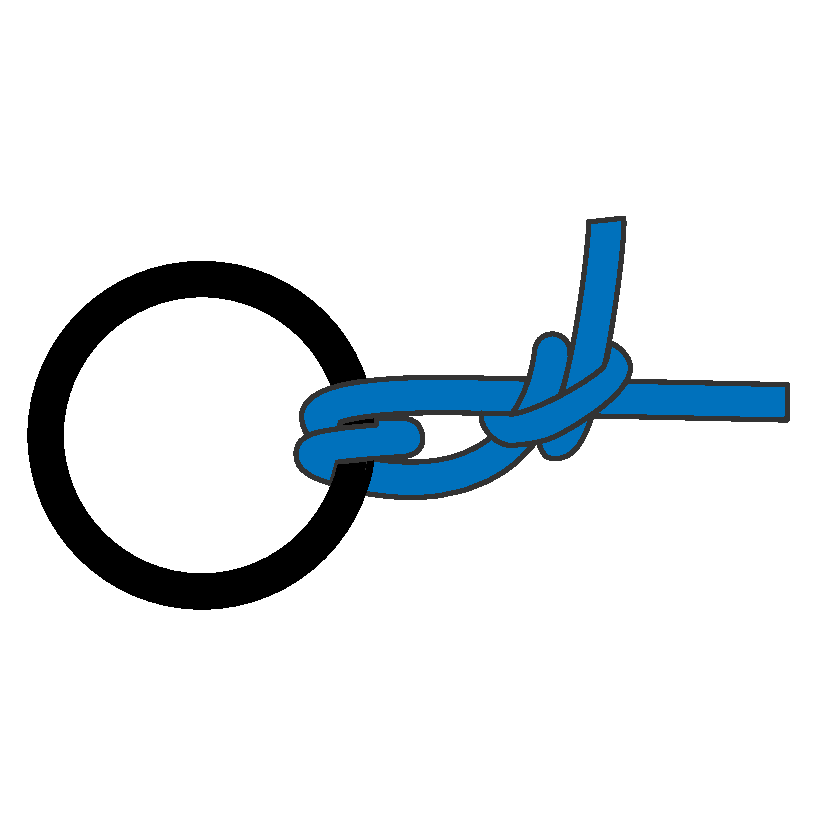
\includegraphics[width=\textwidth]{Hoofdstukken/Schiemannen/pdf/dubble_halve_steek.pdf}
		\centering
		B
	\end{minipage}
	\hfill
	\begin{minipage}[b]{0.23\textwidth}
		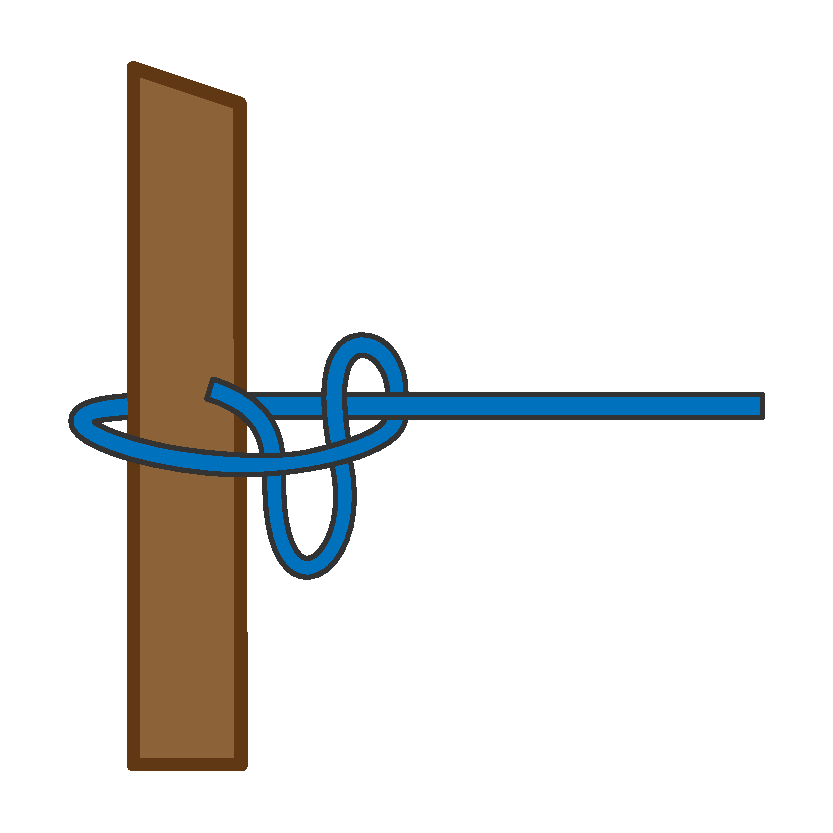
\includegraphics[width=\textwidth]{Hoofdstukken/Schiemannen/pdf/slip_steek.pdf}
		\centering
		C
	\end{minipage}
	\hfill
	\begin{minipage}[b]{0.23\textwidth}
		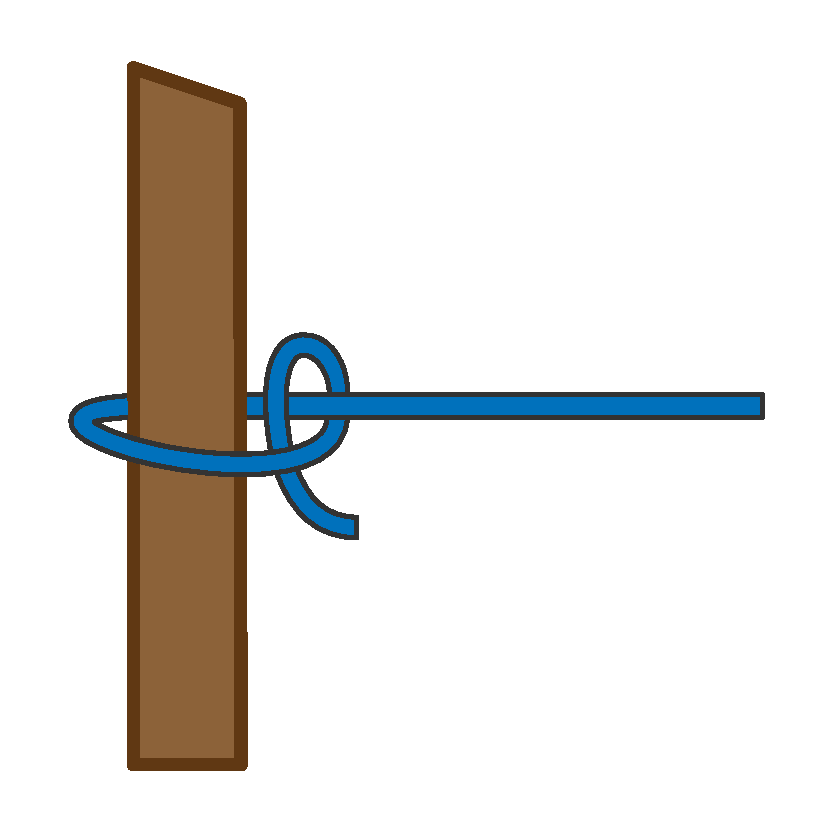
\includegraphics[width=\textwidth]{Hoofdstukken/Schiemannen/pdf/halve_steek.pdf}
		\centering
		D
	\end{minipage}
\end{figure}


\question{5}{Met welke knoop leg je aan een ring vast?}
\answerTextFour{Schootsteek}{Slipsteek}{Dubbele slipsteek}{Dubbele halve steek}
\vspace{0.5cm}
\question{6}{Met welke knoop leg je een verdikking in een touw?}
\answerTextFour{Schootsteek}{Achtknoop}{Knots}{Slipsteek}
